\documentclass[aspectratio=169]{beamer}
\usepackage{will_handley_beamer}
\usepackage{title_page}
\usepackage{hyperref}

\newcommand{\keyterm}[1]{\textbf{\textcolor{C0}{#1}}}

\title{Recent Work}
\date{20\textsuperscript{th} January 2026}

\begin{document}

\begin{frame}
    \titlepage
\end{frame}

% === UNIMPEDED ===

\begin{frame}
    \frametitle{\texttt{unimpeded}: Public Nested Sampling Database}
    \framesubtitle{Ong \& Handley \hfill \arxiv{2511.05470}}
    \student{dily_ong.jpg}{Dily Ong}{PhD Student}
    \vspace{-1em}
    \begin{columns}[T]
        \column{0.55\textwidth}
        \begin{block}{The Problem}
            \begin{itemize}
                \item Model comparison needs \keyterm{Bayesian evidences}
                \item Computing chains is expensive (DiRAC time)
                \item Results often not reproducible or shareable
            \end{itemize}
        \end{block}
        \begin{block}{The Solution: A Public Chain Database}
            \begin{itemize}
                \item \texttt{pip install unimpeded}
                \item 8 cosmological models $\times$ 39 datasets
                \item Pre-computed NS + MCMC chains on Zenodo
                \item Built-in tension statistics (6 metrics)
            \end{itemize}
        \end{block}
        \begin{alertblock}{Like Planck Legacy Archive, but with nested sampling}
            Normalised posteriors + evidences for everyone
        \end{alertblock}
        \column{0.42\textwidth}
        \centering
        \includegraphics[width=\textwidth]{context/arxiv_sources/unimpeded/flowchart.pdf}
    \end{columns}
\end{frame}

\begin{frame}
    \frametitle{\texttt{unimpeded}: Model Comparison Results}
    \framesubtitle{Ong \& Handley \hfill \arxiv{2511.04661}}
    \vspace{-1em}
    \begin{columns}[T]
        \column{0.35\textwidth}
        \begin{block}{Reading the Plot}
            \begin{itemize}
                \item Rows: cosmological models
                \item Columns: datasets
                \item Values: $\log \mathcal{Z}$ (Bayesian evidence)
                \item \textcolor{C0}{Blue}: model disfavoured
                \item \textcolor{C3}{Red}: model favoured
            \end{itemize}
        \end{block}
        \begin{block}{Key Findings}
            \begin{itemize}
                \item $\Lambda$CDM consistently performs well
                \item Extended models penalised by Occam factor
                \item Some tension with CMB lensing
            \end{itemize}
        \end{block}
        \column{0.63\textwidth}
        \centering
        \includegraphics[width=\textwidth,height=0.85\textheight,keepaspectratio]{context/arxiv_sources/unimpeded_grid/figs/model_comparison_single_sorted_by_dkl.pdf}
    \end{columns}
\end{frame}

\begin{frame}
    \frametitle{\texttt{unimpeded}: Tension Quantification Results}
    \framesubtitle{Ong \& Handley \hfill \arxiv{2511.04661}}
    \centering
    \includegraphics[angle=90,height=0.8\textheight,width=0.95\textwidth,keepaspectratio]{context/arxiv_sources/unimpeded_grid/figs/tension_stats_p_sorted_by_p.pdf}
\end{frame}

% === POLYSWYFT ===

\begin{frame}
    \frametitle{\texttt{PolySwyft}: Sequential Simulation-Based Nested Sampling}
    \framesubtitle{Scheutwinkel, Handley, Weniger, de Lera Acedo \hfill \arxiv{2512.08316}}
    \student{kilian_scheutwinkel.jpg}{Kilian Scheutwinkel}{PhD Student}
    \begin{columns}[T]
        \column{0.55\textwidth}
        \begin{block}{The Problem}
            \begin{itemize}
                \item Likelihood often \keyterm{intractable} (simulators only)
                \item Neural Ratio Estimation (NRE) learns likelihood ratios
                \item But: prior truncation struggles with \keyterm{multimodality}
            \end{itemize}
        \end{block}
        \begin{block}{The Solution: Nest NRE inside NS}
            \begin{itemize}
                \item Use nested sampling to explore full likelihood-to-evidence space
                \item Retrain NRE on dead points (active learning)
                \item KL-divergence criterion for convergence
            \end{itemize}
        \end{block}
        \begin{alertblock}{Result}
            Fewer simulator calls than TNRE; handles multimodal posteriors; applied to CMB with \texttt{CosmoPower}
        \end{alertblock}
        \column{0.42\textwidth}
        \centering
        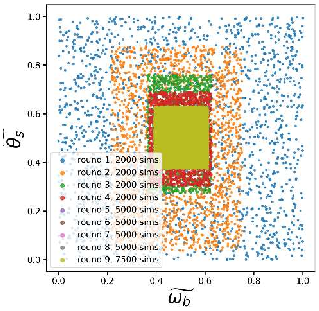
\includegraphics[width=\textwidth]{figures/tmnre.pdf}
    \end{columns}
\end{frame}

\begin{frame}
    \frametitle{\texttt{PolySwyft}: The NSNRE Algorithm}
    \framesubtitle{Scheutwinkel, Handley, Weniger, de Lera Acedo \hfill \arxiv{2512.08316}}
    \student{kilian_scheutwinkel.jpg}{Kilian Scheutwinkel}{PhD Student}
    \centering
    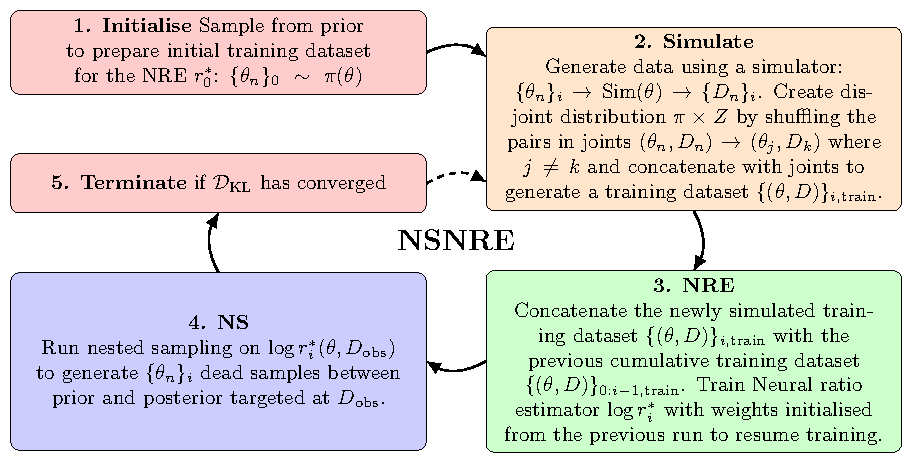
\includegraphics[width=0.85\textwidth,height=0.8\textheight,keepaspectratio]{figures/polyswyft_flowchart.pdf}
\end{frame}

\end{document}
